\subsection{Architektur\label{subsec:architektur}}

\subsubsection{Übersicht}
\begin{wrapfigure}{l}{.5\textwidth}
	\centering
	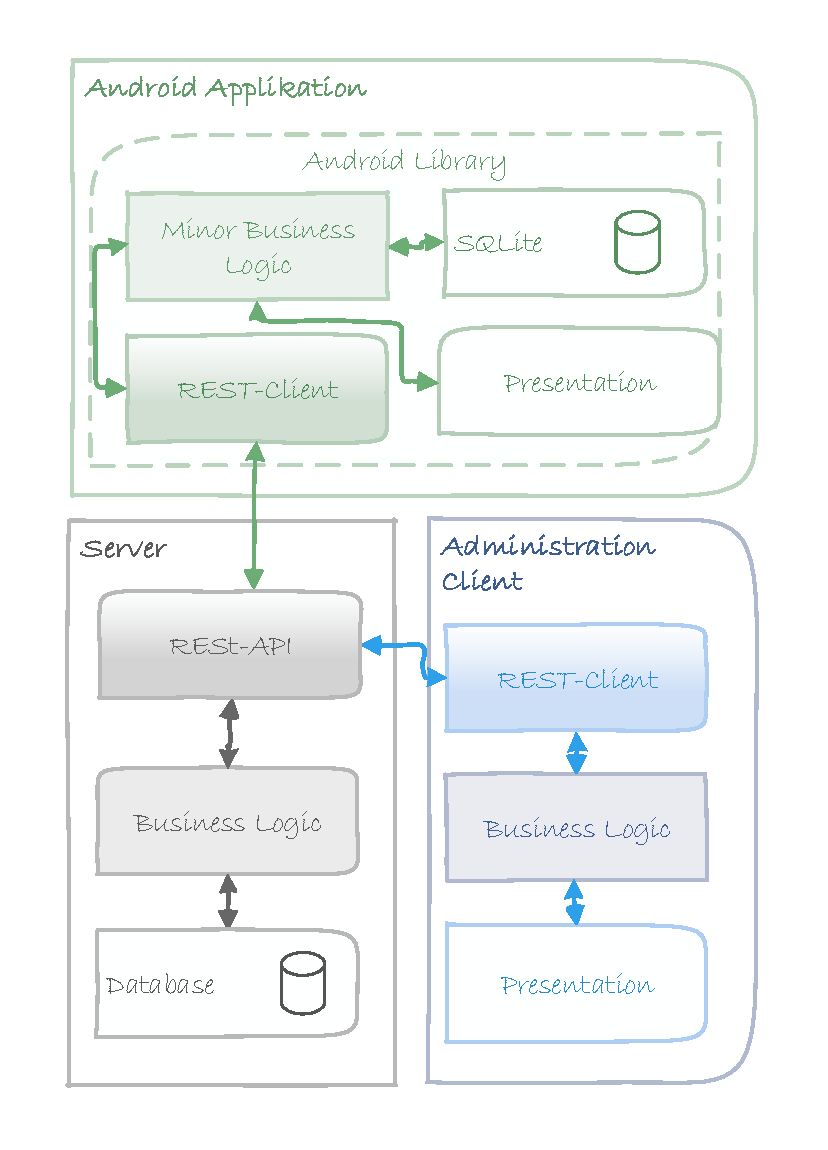
\includegraphics[width=\linewidth]{img/architecture_draft}
	\caption{Architektur des Frameworks (Entwurf).}
	\label{fig:architektur_entwurf}
\end{wrapfigure}
Das Framework ist in drei Komponenten unterteilt: Server, Android Bibliothek und ein Client für Testleiter~/~Administratoren.

\subsubsection{Server}
Der Aufbau der Komponenten ist in Abbildung \ref{fig:architektur_entwurf} dargestellt.
Die Kommunikation zwischen den Komponenten erfolgt per \ac{HTTP} und eine \ac{REST}-\ac{API}.
Der Server nutzt zur Datenhaltung eine Datenbank, auf welche durch die Geschäftslogik zugegriffen wird.
%TODO weiterschreiben oder zusammenfassen.

\subsubsection{Android-Biliothek}

\subsubsection{Administrations-Client}